

%🍁% \chapter{Strings  |  字符串}
\chapter{字符串}
\label{strings}

%🍁% Strings are not like integers, floats, and booleans.  A string
%🍁% is a {\bf sequence}, which means it is
%🍁% an ordered collection of other values.  In this chapter you'll see
%🍁% how to access the characters that make up a string, and you'll
%🍁% learn about some of the methods strings provide.
%🍁% \index{sequence}

字符串不像整数、浮点数和布尔型。 字符串是一个 {\em 序列} (sequence) ,这就意味着
它是其他值的一个有序的集合。 在这章中,你将学习怎么去访问字符串里的字符, 同时你也会学习到字符串提供的一些方法。
\index{sequence}

%🍁% \section{A string is a sequence  |  字符串是一个序列}
\section{字符串是一个序列}

\index{sequence}  \index{character}
\index{bracket operator}  \index{operator!bracket}

%🍁% A string is a sequence of characters.
%🍁% You can access the characters one at a time with the
%🍁% bracket operator:

字符串是由字符组成的序列。 你可以用括号运算符一次访问一个字符:

\begin{lstlisting}
>>> fruit = 'banana'
>>> letter = fruit[1]
\end{lstlisting}

%
%🍁% The second statement selects character number 1 from {\tt
%🍁% fruit} and assigns it to {\tt letter}.
\index{index}

第2条语句从 \li{fruit} 中选择索引为1的字符并将它赋给 \li{letter} 。

%🍁% The expression in brackets is called an {\bf index}.
%🍁% The index indicates which character in the sequence you
%🍁% want (hence the name).

括号中的表达式被称作 {\em 索引} (index)。 索引指出在序列中你想要哪个字符(因此而得名)。

%🍁% But you might not get what you expect:

但是你可能不会获得你期望的东西:

\begin{lstlisting}
>>> letter
'a'
\end{lstlisting}

%
%🍁% For most people, the first letter of \verb"'banana'" is {\tt b}, not
%🍁% {\tt a}.  But for computer scientists, the index is an offset from the
%🍁% beginning of the string, and the offset of the first letter is zero.

对于大多数人,\li{'banana'} 的第一个字母是 \li{b} 而不是 \li{a}。
但是对于计算机科学家,索引是从字符串起点开始的位移量 (offset) ,第一个字母的位移量就是 0。

\begin{lstlisting}
>>> letter = fruit[0]
>>> letter
'b'
\end{lstlisting}

%
%🍁% So {\tt b} is the 0th letter (``zero-eth'') of \verb"'banana'", {\tt
%🍁%   a} is the 1th letter (``one-eth''), and {\tt n} is the 2th letter
%🍁% (``two-eth'').  \index{index!starting at zero} \index{zero, index
%🍁%   starting at}

所以 \li{b} 是 \li{'banana'} 的第 $0$ 个字母, \li {a} 是第一个字母, \li{n} 是第二个字母\footnote{译注:原文分别是 ``zero-eth'', ``one-eth'', ``two-eth''}。

%🍁% As an index you can use an expression that contains variables and
%🍁% operators:
\index{index}

你可以使用一个包含变量名和运算符的表达式作为索引:

\begin{lstlisting}
>>> i = 1
>>> fruit[i]
'a'
>>> fruit[i+1]
'n'
\end{lstlisting}

%

%🍁% But the value of the index has to be an integer.  Otherwise you
%🍁% get:
\index{exception!TypeError}  \index{TypeError}

索引值必须使用整数。 否则你会得到报错:

\begin{lstlisting}
>>> letter = fruit[1.5]
TypeError: string indices must be integers
\end{lstlisting}


%
%🍁% \section{{\tt len}}
\section{{\tt len}}
\index{len function}  \index{function!len}

%🍁% {\tt len} is a built-in function that returns the number of characters
%🍁% in a string:

\li{len} 是一个内建函数,它返回字符串中的字符的数量:

\begin{lstlisting}
>>> fruit = 'banana'
>>> len(fruit)
6
\end{lstlisting}

%
%🍁% To get the last letter of a string, you might be tempted to try something
%🍁% like this:
\index{exception!IndexError}  \index{IndexError}

为了获得某个字符串中最后一个字符,你可以尝试这样操作:

\begin{lstlisting}
>>> length = len(fruit)
>>> last = fruit[length]
IndexError: string index out of range
\end{lstlisting}

%
%🍁% The reason for the {\tt IndexError} is that there is no letter in {\tt
%🍁% 'banana'} with the index 6.  Since we started counting at zero, the
%🍁% six letters are numbered 0 to 5.  To get the last character, you have
%🍁% to subtract 1 from {\tt length}:

出现 \li{IndexError} 的原因在于 \li{'banana'} 中没有索引值为 6 的字母。 由于我们从 0 开始计数,六个字母的编号是从 0 到 5 。 为了获得最后一个字符,你必须将 、力{length} 减去一:

\begin{lstlisting}
>>> last = fruit[length-1]
>>> last
'a'
\end{lstlisting}

%
%🍁% Or you can use negative indices, which count backward from
%🍁% the end of the string.  The expression {\tt fruit[-1]} yields the last
%🍁% letter, {\tt fruit[-2]} yields the second to last, and so on.
\index{index!negative}  \index{negative index}

你也可以使用负数索引,即从字符串的末尾倒着往前数。 表达式 \li{fruit[-1]} 返回的是最后一个字母, \li{fruit[-2]} 返回倒数第二个字母, 以此类推。
\index{index!negative}  \index{negative index}
\index{index!negative}  \index{negative index}


%🍁% \section{Traversal with a {\tt for} loop  |  使用{\tt for}循环遍历}
\section{使用{\tt for}循环遍历}
\label{for}
\index{traversal}  \index{loop!traversal}
\index{for loop}  \index{loop!for}
\index{statement!for}  \index{traversal}

%🍁% A lot of computations involve processing a string one character at a
%🍁% time.  Often they start at the beginning, select each character in
%🍁% turn, do something to it, and continue until the end.  This pattern of
%🍁% processing is called a {\bf traversal}.  One way to write a traversal
%🍁% is with a {\tt while} loop:

许多计算中需要一个字符一个字符地处理字符串。 通常计算从字符串的头部开始,依次选择每个字符,对其做一些处理,
然后继续直到结束。 这种处理模式被称作 {\em 遍历} (traversal) 。 编写遍历的方法之一是使用 \li{while} 循环:


\begin{lstlisting}
index = 0
while index < len(fruit):
    letter = fruit[index]
    print(letter)
    index = index + 1
\end{lstlisting}

%
%🍁% This loop traverses the string and displays each letter on a line by
%🍁% itself.  The loop condition is {\tt index < len(fruit)}, so
%🍁% when {\tt index} is equal to the length of the string, the
%🍁% condition is false, and the body of the loop doesn't run.  The
%🍁% last character accessed is the one with the index {\tt len(fruit)-1},
%🍁% which is the last character in the string.

该循环遍历字符串并在每行显示一个字符串。 该循环的条件是 \li{index < len(fruit)}, 所以当 \li{index} 和字符串的长度相等时, 条件为假, 循环体不被执行。 被访问的最后一个字符的索引为 \li{len(fruit)-1}, 这也是字符串的最后一个字符。

%🍁% As an exercise, write a function that takes a string as an argument
%🍁% and displays the letters backward, one per line.

我们做个练习,编写一个函数,接受一个字符串作为实参,
按照从后向前的顺序显示字符,每行只显示一个。

%🍁% Another way to write a traversal is with a {\tt for} loop:

编写遍历的另一种方法是使用 \li{for} 循环:

\begin{lstlisting}
for letter in fruit:
    print(letter)
\end{lstlisting}

%
%🍁% Each time through the loop, the next character in the string is assigned
%🍁% to the variable {\tt letter}.  The loop continues until no characters are
%🍁% left.
\index{concatenation}  \index{abecedarian}
\index{McCloskey, Robert}

每次循环时,字符串中的下一个字符被赋值给变量 \li{letter} 。 循环继续,直到没有剩余的字符串了。

%🍁% The following example shows how to use concatenation (string addition)
%🍁% and a {\tt for} loop to generate an abecedarian series (that is, in
%🍁% alphabetical order).  In Robert McCloskey's book {\em Make
%🍁% Way for Ducklings}, the names of the ducklings are Jack, Kack, Lack,
%🍁% Mack, Nack, Ouack, Pack, and Quack.  This loop outputs these names in
%🍁% order:

下面的例子演示了如何使用拼接(字符串相加)和 \li{for} 循环生成一个字母表序列 (即按照字母表顺序排列)。 在 Robert McCloskey 的书 《{\em Make Way for Ducklings}》 中, 小鸭子的名字是 Jack、 Kack、 Lack、 Mack、 Nack、 Ouack、 Pack 和 Quack。 此循环按顺序输出这些名字:
\index{concatenation}

\begin{lstlisting}
prefixes = 'JKLMNOPQ'
suffix = 'ack'

for letter in prefixes:
    print(letter + suffix)
\end{lstlisting}

%
The output is:
输出是:

\begin{lstlisting}
Jack
Kack
Lack
Mack
Nack
Oack
Pack
Qack
\end{lstlisting}

%
%🍁% Of course, that's not quite right because ``Ouack'' and ``Quack'' are
%🍁% misspelled.  As an exercise, modify the program to fix this error.

当然,输出并不完全正确,因为 ``Ouack'' 和 ``Quack'' 拼写错了。我们做个练习, 修改这个程序,解决这个问题。


%🍁% \section{String slices  |  字符串切片}
\section{字符串切片}
\label{slice}
\index{slice operator} \index{operator!slice} \index{index!slice}
\index{string!slice} \index{slice!string}

%🍁% A segment of a string is called a {\bf slice}.  Selecting a slice is
%🍁% similar to selecting a character:

字符串的一个片段被称作 {\em 切片} (slice)。 选择一个切片的操作类似于选择一个字符:

\begin{lstlisting}
>>> s = 'Monty Python'
>>> s[0:5]
'Monty'
>>> s[6:12]
'Python'
\end{lstlisting}

%
%🍁% The operator {\tt [n:m]} returns the part of the string from the
%🍁% ``n-eth'' character to the ``m-eth'' character, including the first but
%🍁% excluding the last.  This behavior is counterintuitive, but it might
%🍁% help to imagine the indices pointing {\em between} the
%🍁% characters, as in Figure~\ref{fig.banana}.

操作符 \li{[n:m]} 返回从第 n 个字符到第 m 个字符的字符串片段, 包括第一个, 但是不包括最后一个。 这个行为违反直觉, 但是将指向两个字符之间的索引, 想象成图~ \ref{fig.banana} 中那样或许有帮助。

\begin{figure}
\centerline
{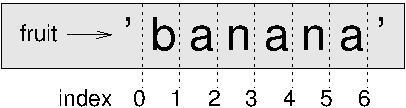
\includegraphics[scale=0.8]{../source/figs/banana.pdf}}
% \caption{Slice indices.}
\caption{切片索引。}
\label{fig.banana}
\end{figure}

%🍁% If you omit the first index (before the colon), the slice starts at
%🍁% the beginning of the string.  If you omit the second index, the slice
%🍁% goes to the end of the string:

如果你省略第一个索引(冒号前面的值), 切片起始于字符串头部。 如果你省略第二个索引,切片一直到字符串结尾:

\begin{lstlisting}
>>> fruit = 'banana'
>>> fruit[:3]
'ban'
>>> fruit[3:]
'ana'
\end{lstlisting}

%
%🍁% If the first index is greater than or equal to the second the result
%🍁% is an {\bf empty string}, represented by two quotation marks:
%🍁% \index{quotation mark}

如果第一个索引大于或等于第二个,结果是 {\em 空字符串} (empty string) , 用两个引号表示:

\begin{lstlisting}
>>> fruit = 'banana'
>>> fruit[3:3]
''
\end{lstlisting}

%
%🍁% An empty string contains no characters and has length 0, but other
%🍁% than that, it is the same as any other string.

一个空字符串不包括字符而且长度为 0,但除此之外, 它和其它任何字符串一样。

%🍁% Continuing this example, what do you think
%🍁% {\tt fruit[:]} means?  Try it and see.
\index{copy!slice}  \index{slice!copy}


%🍁% \section{Strings are immutable  |  字符串是不可变的}
\section{字符串是不可变的}
\index{mutability}  \index{immutability}  \index{string!immutable}

%🍁% It is tempting to use the {\tt []} operator on the left side of an
%🍁% assignment, with the intention of changing a character in a string.
%🍁% For example:
%🍁% \index{TypeError}  \index{exception!TypeError}

你会很想在赋值语句的左边使用 \li{[]}, 来改变字符串的一个字符。 例如:
\index{TypeError}  \index{exception!TypeError}

\begin{lstlisting}
>>> greeting = 'Hello, world!'
>>> greeting[0] = 'J'
TypeError: 'str' object does not support item assignment
\end{lstlisting}

%
%🍁% The ``object'' in this case is the string and the ``item'' is
%🍁% the character you tried to assign.  For now, an object is
%🍁% the same thing as a value, but we will refine that definition
%🍁% later (Section~\ref{equivalence}).
\index{object}  \index{item}  \index{item assignment}
\index{assignment!item}  \index{immutability}

错误信息中的 ``object(对象)'' 是那个字符串,``item(元素)''是你要赋值的字符。 目前, 我们认为对象和值是同样的东西, 但是我们后面将改进此定义 (详见 \hyperref[equivalence]{对象与值}一节)。

%🍁% The reason for the error is that
%🍁% strings are {\bf immutable}, which means you can't change an
%🍁% existing string.  The best you can do is create a new string
%🍁% that is a variation on the original:

出现此错误的原因是字符串是 {\em 不可变的} (immutable), 这意味着你不能改变一个已存在的字符串。 你最多只能创建一个新的字符串,在原有字符串的基础上略有变化:

\begin{lstlisting}
>>> greeting = 'Hello, world!'
>>> new_greeting = 'J' + greeting[1:]
>>> new_greeting
'Jello, world!'
\end{lstlisting}

%
%🍁% This example concatenates a new first letter onto
%🍁% a slice of {\tt greeting}.  It has no effect on
%🍁% the original string.
\index{concatenation}

上面的示例中, 我们将一个新的首字母拼接到 \li{greeting} 的一个切片上。 它不影响原字符串。


%🍁% \section{Searching  |  搜索}
\section{搜索}
\label{find}

%🍁% What does the following function do?
\index{find function}  \index{function!find}

下面的函数起什么作用?

\begin{lstlisting}
def find(word, letter):
    index = 0
    while index < len(word):
        if word[index] == letter:
            return index
        index = index + 1
    return -1
\end{lstlisting}

%
%🍁% In a sense, {\tt find} is the inverse of the {\tt []} operator.
%🍁% Instead of taking an index and extracting the corresponding character,
%🍁% it takes a character and finds the index where that character
%🍁% appears.  If the character is not found, the function returns {\tt
%🍁% -1}.

在某种意义上,\li{find} 和 \li{[]} 运算符相反。 与接受一个索引并提取相应的字符不同, 它接受一个字符并找到该字符所在的索引。 如果没有找到该字符, 函数返回 \li{-1}。

%🍁% This is the first example we have seen of a {\tt return} statement
%🍁% inside a loop.  If {\tt word[index] == letter}, the function breaks
%🍁% out of the loop and returns immediately.

这是我们第一次在循环内部看见 \li{return} 语句。如果 \li{word[index] == letter},
函数停止循环并马上返回。

%🍁% If the character doesn't appear in the string, the program
%🍁% exits the loop normally and  returns {\tt -1}.

如果字符没出现在字符串中,那么程序正常退出循环并返回 \li{-1}。

%🍁% This pattern of computation---traversing a sequence and returning
%🍁% when we find what we are looking for---is called a {\bf search}.
\index{traversal}  \index{search pattern}  \index{pattern!search}

这种计算模式——遍历一个序列并在找到寻找的东西时返回——被称作 {\em 搜索} (search)。

%🍁% As an exercise, modify {\tt find} so that it has a
%🍁% third parameter, the index in {\tt word} where it should start
%🍁% looking.

我们做个练习,修改 \li {find} 函数使得它能接受第三个参数, 即从何处开始搜索的索引。

%🍁% \section{Looping and counting  |  循环和计数}
\section{循环和计数}
\label{counter}
\index{counter}  \index{counting and looping}
\index{looping and counting}  \index{looping!with strings}

%🍁% The following program counts the number of times the letter {\tt a}
%🍁% appears in a string:

下面的程序计算字母a在字符串中出现的次数:

\begin{lstlisting}
word = 'banana'
count = 0
for letter in word:
    if letter == 'a':
        count = count + 1
print(count)
\end{lstlisting}

%
%🍁% This program demonstrates another pattern of computation called a {\bf
%🍁% counter}.  The variable {\tt count} is initialized to 0 and then
%🍁% incremented each time an {\tt a} is found.
%🍁% When the loop exits, {\tt count}
%🍁% contains the result---the total number of {\tt a}'s.

此程序演示了另一种被称作 {\em 计数器} (counter) 的计算模式。变量 \li{count} 初始化为 0 , 然后每次出现 \li{a} 时递增。当循环结束时,\li{count} 包含了字母 \li{a} 出现的总次数。

\index{encapsulation}
%🍁% As an exercise, encapsulate this code in a function named {\tt
%🍁% count}, and generalize it so that it accepts the string and the
%🍁% letter as arguments.

我们做一个练习, 将这段代码封装在一个名为 \li{count} 的函数中, 并泛化该函数, 使其接受字符串和字母作为实参。

%🍁% Then rewrite the function so that instead of
%🍁% traversing the string, it uses the three-parameter version of {\tt
%🍁% find} from the previous section.

然后重写这个函数, 不再使用字符串遍历, 而是使用上一节中三参数版本的 \li{find} 函数。

%🍁% \section{String methods  |  字符串方法}
\section{字符串方法}
\label{optional}

%🍁% Strings provide methods that perform a variety of useful operations.
%🍁% A method is similar to a function---it takes arguments and
%🍁% returns a value---but the syntax is different.  For example, the
%🍁% method {\tt upper} takes a string and returns a new string with
%🍁% all uppercase letters.
\index{method}  \index{string!method}

字符串提供了可执行多种有用操作的 {\em 方法} (method) 。 方法和函数类似, 接受实参并返回一个值, 但是语法不同。 例如,\li{upper} 方法接受一个字符串, 并返回一个都是大写字母的新字符串。

%🍁% Instead of the function syntax {\tt upper(word)}, it uses
%🍁% the method syntax {\tt word.upper()}.

不过使用的不是函数语法 \li{upper(word)} , 而是方法的语法 \li{word.upper()}。

\begin{lstlisting}
>>> word = 'banana'
>>> new_word = word.upper()
>>> new_word
'BANANA'
\end{lstlisting}

%
%🍁% This form of dot notation specifies the name of the method, {\tt
%🍁% upper}, and the name of the string to apply the method to, {\tt
%🍁% word}.  The empty parentheses indicate that this method takes no
%🍁% arguments.
\index{parentheses!empty}  \index{dot notation}

点标记法的形式指出方法的名字,\li{upper},以及应用该方法的字符串的名字,\li{word}。 空括号表明该方法不接受实参。

%🍁% A method call is called an {\bf invocation}; in this case, we would
%🍁% say that we are invoking {\tt upper} on {\tt word}.
\index{invocation}

这被称作 {\em 方法调用} (invocation); 此例中, 我们可以说是在 \li{word} 上调用 \li{upper} 。

%🍁% As it turns out, there is a string method named {\tt find} that
%🍁% is remarkably similar to the function we wrote:

事实上,有一个被称为 \li{find} 的字符串方法, 与我们之前写的函数极其相似:

\begin{lstlisting}
>>> word = 'banana'
>>> index = word.find('a')
>>> index
1
\end{lstlisting}

%
%🍁% In this example, we invoke {\tt find} on {\tt word} and pass
%🍁% the letter we are looking for as a parameter.

此例中,我们在 \li{word} 上调用 \li{find} ,并将我们要找的字母作为参数传入。

%🍁% Actually, the {\tt find} method is more general than our function;
%🍁% it can find substrings, not just characters

事实上, \li{find} 方法比我们的函数更通用; 它还可以查找子字符串, 而不仅仅是字符:

\begin{lstlisting}
>>> word.find('na')
2
\end{lstlisting}

%
%🍁% By default, {\tt find} starts at the beginning of the string, but
%🍁% it can take a second argument, the index where it should start:
\index{optional argument}  \index{argument!optional}

\li{find} 默认从字符串的首字母开始查找, 它还可以接受第二个实参, 即从何处开始的索引。

\begin{lstlisting}
>>> word.find('na', 3)
4
\end{lstlisting}

%
%🍁% This is an example of an {\bf optional argument};
%🍁% {\tt find} can
%🍁% also take a third argument, the index where it should stop:

这是一个 {\em 可选参数} (optional argument) 的例子; \li{find} 也可以接受结束查找的索引作为第三个实参:

\begin{lstlisting}
>>> name = 'bob'
>>> name.find('b', 1, 2)
-1
\end{lstlisting}

%
%🍁% This search fails because {\tt b} does not
%🍁% appear in the index range from {\tt 1} to {\tt 2}, not including {\tt
%🍁% 2}.  Searching up to, but not including, the second index makes
%🍁% {\tt find} consistent with the slice operator.

此次搜索失败,因为 \li{'b'} 没有出现在索引 \li{1}--\li{2} 之间(不包括\li{2})。 一直搜索到第二个索引,但是并不搜索第二个索引, 这使得 \li{find} 跟切片运算符的行为一致.

%🍁% \section{The {\tt in} operator  |  {\tt in} 运算符}
\section{{\tt in} 运算符}
\label{inboth}
\index{in operator}  \index{operator!in}
\index{boolean operator}  \index{operator!boolean}

%🍁% The word {\tt in} is a boolean operator that takes two strings and
%🍁% returns {\tt True} if the first appears as a substring in the second:

单词 \li{in} 是一个布尔运算符, 接受两个字符串。 如果第一个作为子串出现在第二个中, 则返回 \li{True}:

\begin{lstlisting}
>>> 'a' in 'banana'
True
>>> 'seed' in 'banana'
False
\end{lstlisting}

%
%🍁% For example, the following function prints all the
%🍁% letters from {\tt word1} that also appear in {\tt word2}:

例如,下面的函数打印所有既出现在 \li{word1} 中,也出现在 \li{word2} 中的字母:

\begin{lstlisting}
def in_both(word1, word2):
    for letter in word1:
        if letter in word2:
            print(letter)
\end{lstlisting}

%
%🍁% With well-chosen variable names,
%🍁% Python sometimes reads like English.  You could read
%🍁% this loop, ``for (each) letter in (the first) word, if (the) letter
%🍁% (appears) in (the second) word, print (the) letter.''

变量名挑选得当的话, Python 代码有时候读起来像是自然语言。 你可以这样读此循环, ``对于(每个) 在(第一个)单词中的字母,如果(该)字母(出现)在(第二个)单词中,打印(该)字母''。

%🍁% Here's what you get if you compare apples and oranges:

如果你比较 \li{'apples'} 和 \li{'oranges'},你会得到下面的结果:

\begin{lstlisting}
>>> in_both('apples', 'oranges')
a
e
s
\end{lstlisting}

%

%🍁% \section{String comparison  |  字符串比较}
\section{字符串比较}
\index{string!comparison}  \index{comparison!string}

%🍁% The relational operators work on strings.  To see if two strings are equal:

关系运算符也适用于字符串。可以这样检查两个字符串是否相等:

\begin{lstlisting}
if word == 'banana':
    print('All right, bananas.')
\end{lstlisting}

%
%🍁% Other relational operations are useful for putting words in alphabetical
%🍁% order:

其它的关系运算符对于按字母序放置单词也很有用:

\begin{lstlisting}
if word < 'banana':
    print('Your word, ' + word + ', comes before banana.')
elif word > 'banana':
    print('Your word, ' + word + ', comes after banana.')
else:
    print('All right, bananas.')
\end{lstlisting}

%
%🍁% Python does not handle uppercase and lowercase letters the same way
%🍁% people do.  All the uppercase letters come before all the
%🍁% lowercase letters, so:

Python处理大写和小写字母的方式和人不同。所有的大写字母出现在所有小写字母之前,所以:

\begin{lstlisting}
Your word, Pineapple, comes before banana.
\end{lstlisting}

%
%🍁% A common way to address this problem is to convert strings to a
%🍁% standard format, such as all lowercase, before performing the
%🍁% comparison. Keep that in mind in case you have to defend yourself
%🍁% against a man armed with a Pineapple.

%🍁% \section{Debugging  |  调试}
\section{调试}
\index{debugging}  \index{traversal}

%🍁% When you use indices to traverse the values in a sequence,
%🍁% it is tricky to get the beginning and end of the traversal
%🍁% right.  Here is a function that is supposed to compare two
%🍁% words and return {\tt True} if one of the words is the reverse
%🍁% of the other, but it contains two errors:

当你使用索引遍历序列中的值时,正确地指定遍历的起始和结束点有点困难。下面是一个用来比较两个单词的函数,如果一个单词是另一个的倒序,则返回 \li{True} , 但其中有两个错误:

\begin{lstlisting}
def is_reverse(word1, word2):
    if len(word1) != len(word2):
        return False

    i = 0
    j = len(word2)

    while j > 0:
        if word1[i] != word2[j]:
            return False
        i = i+1
        j = j-1

    return True
\end{lstlisting}

%
%🍁% The first {\tt if} statement checks whether the words are the
%🍁% same length.  If not, we can return {\tt False} immediately.
%🍁% Otherwise, for the rest of the function, we can assume that the words
%🍁% are the same length.  This is an example of the guardian pattern
%🍁% in Section~\ref{guardian}.
\index{guardian pattern}  \index{pattern!guardian}
\index{index}

第一条 \li{if} 语句检查两个单词是否等长。如果不是,我们可以马上返回 \li{False} 。否则,在函数其余的部分,我们可以假定单词是等长的。这是~\ref{guardian}节中提到的监护人模式的一个例子。

%🍁% {\tt i} and {\tt j} are indices: {\tt i} traverses {\tt word1}
%🍁% forward while {\tt j} traverses {\tt word2} backward.  If we find
%🍁% two letters that don't match, we can return {\tt False} immediately.
%🍁% If we get through the whole loop and all the letters match, we
%🍁% return {\tt True}.

\li{i} 和 \li{j} 是索引:\li{i} 向前遍历 \li{word1},\li{j} 向后遍历 \li{word2}。 如果我们找到两个不匹配的字母, 我们可以立即返回 \li{False}。 如果我们完成整个循环并且所有字母都匹配,我们返回 \li{True} 。

%🍁% If we test this function with the words ``pots'' and ``stop'', we
%🍁% expect the return value {\tt True}, but we get an IndexError:
\index{IndexError}  \index{exception!IndexError}

如果我们用单词 ``pots'' 和 ``stop'' 测试该函数, 我们期望返回 \li{True} , 但是却得到一个 \li{IndexError}:

\begin{lstlisting}
>>> is_reverse('pots', 'stop')
...
  File "reverse.py", line 15, in is_reverse
    if word1[i] != word2[j]:
IndexError: string index out of range
\end{lstlisting}

%
%🍁% For debugging this kind of error, my first move is to
%🍁% print the values of the indices immediately before the line
%🍁% where the error appears.

为了调试该类错误, 我第一步是在错误出现的行之前,打印索引的值。

\begin{lstlisting}
    while j > 0:
        print(i, j)        # print here

        if word1[i] != word2[j]:
            return False
        i = i+1
        j = j-1
\end{lstlisting}

%
%🍁% Now when I run the program again, I get more information:

现在,当我再次运行该程序时,将获得更多的信息:

\begin{lstlisting}
>>> is_reverse('pots', 'stop')
0 4
...
IndexError: string index out of range
\end{lstlisting}

%
%🍁% The first time through the loop, the value of {\tt j} is 4,
%🍁% which is out of range for the string \verb"'pots'".
%🍁% The index of the last character is 3, so the
%🍁% initial value for {\tt j} should be {\tt len(word2)-1}.

第一次循环时, \li{j} 的值是4, 超出字符串 \li{'post'} 的范围了。 最后一个字符的索引是 \li{3},所以 \li{j} 的初始值应该是 \li{len(word2)-1} 。

%🍁% If I fix that error and run the program again, I get:

如果我解决了这个错误,然后运行程序, 将获得如下输出:

\begin{lstlisting}
>>> is_reverse('pots', 'stop')
0 3
1 2
2 1
True
\end{lstlisting}

%
%🍁% This time we get the right answer, but it looks like the loop only ran
%🍁% three times, which is suspicious.  To get a better idea of what is
%🍁% happening, it is useful to draw a state diagram.  During the first
%🍁% iteration, the frame for \verb"is_reverse" is shown in
%🍁% Figure~\ref{fig.state4}.  \index{state diagram} \index{diagram!state}

这次我们获得了正确的答案,但是看起来循环只运行了三次,这很奇怪。画栈图可以帮我们更好的理解发生了什么。在第一次迭代期间, \li{is_reverse} 的栈帧如图~\ref{fig.state4} 所示。

\begin{figure}
\centerline
{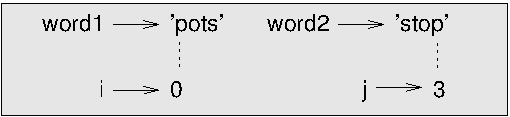
\includegraphics[scale=0.8]{../source/figs/state4.pdf}}
% \caption{State diagram.}
\caption{堆栈图。}
\label{fig.state4}
\end{figure}

%🍁% I took some license by arranging the variables in the frame
%🍁% and adding dotted lines to show that the values of {\tt i} and
%🍁% {\tt j} indicate characters in {\tt word1} and {\tt word2}.

我对堆栈图做了些调整,重新排列了栈帧中的变量,增加了虚线来说明 \li{i} 和 \li{j} 的值表示 \li{word1} 和 \li{word2} 中的字符。


%🍁% Starting with this diagram, run the program on paper, changing the
%🍁% values of {\tt i} and {\tt j} during each iteration.  Find and fix the
%🍁% second error in this function.

从这个堆栈图开始,在纸上运行程序,每次迭代时修改 \li{i} 和 \li{j} 的值。 查找并解决这个函数的中第二个错误。
\label{isreverse}


%🍁% \section{Glossary  |  术语表}
\section{术语表}

%🍁% \begin{description}
%🍁%
%🍁% \item[object:] Something a variable can refer to.  For now,
%🍁% you can use ``object'' and ``value'' interchangeably.
%🍁% \index{object}
%🍁%
%🍁% \item[sequence:] An ordered collection of
%🍁% values where each value is identified by an integer index.
%🍁% \index{sequence}
%🍁%
%🍁% \item[item:] One of the values in a sequence.
%🍁% \index{item}
%🍁%
%🍁% \item[index:] An integer value used to select an item in
%🍁% a sequence, such as a character in a string.  In Python
%🍁% indices start from 0.
%🍁% \index{index}
%🍁%
%🍁% \item[slice:] A part of a string specified by a range of indices.
%🍁% \index{slice}
%🍁%
%🍁% \item[empty string:] A string with no characters and length 0, represented
%🍁% by two quotation marks.
%🍁% \index{empty string}
%🍁%
%🍁% \item[immutable:] The property of a sequence whose items cannot
%🍁% be changed.
%🍁% \index{immutability}
%🍁%
%🍁% \item[traverse:] To iterate through the items in a sequence,
%🍁% performing a similar operation on each.
%🍁% \index{traversal}
%🍁%
%🍁% \item[search:] A pattern of traversal that stops
%🍁% when it finds what it is looking for.
%🍁% \index{search pattern}
%🍁% \index{pattern!search}
%🍁%
%🍁% \item[counter:] A variable used to count something, usually initialized
%🍁% to zero and then incremented.
%🍁% \index{counter}
%🍁%
%🍁% \item[invocation:] A statement that calls a method.
%🍁% \index{invocation}
%🍁%
%🍁% \item[optional argument:] A function or method argument that is not
%🍁% required.
%🍁% \index{optional argument}
%🍁% \index{argument!optional}
%🍁%
%🍁% \end{description}

\begin{description}

\item[对象 (object):] 变量可以引用的东西。现在你将对象和值等价使用。
\index{object}

\item[序列 (sequence):] 一个有序的值的集合,每个值通过一个整数索引标识。
\index{sequence}

\item[元素 (item):] 序列中的一个值。
\index{item}

\item[索引 (index):] 用来选择序列中元素 (如字符串中的字符) 的一个整数值。 在Python中,索引从0开始。
\index{index}

\item[切片 (slice):] 以索引范围指定的字符串片段。
\index{slice}

\item[空字符串 (empty string):] 一个没有字符的字符串,长度为0,用两个引号表示。
\index{empty string}

\item[不可变性 (immutable)] 元素不能被改变的序列的性质。
\index{immutability}

\item[遍历 (traversal):] 对一个序列的所有元素进行迭代, 对每一元素执行类似操作。
\index{traversal}

\item[搜索 (search):] 一种遍历模式,当找到搜索目标时就停止。
\index{search pattern}  \index{pattern!search}

\item[计数器 (counter):] 用来计数的变量,通常初始化为0,并以此递增。
\index{counter}

\item[方法调用(invocation):] 执行一个方法的声明.
\index{invocation}

\item[可选参数 (optional argument):] 一个函数或者一个方法中不必要指定的参数。
\index{optional argument}  \index{argument!optional}

\end{description}


%🍁% \section{Exercises  |  练习}
\section{练习}

\begin{exercise}
\index{string method}  \index{method!string}

%🍁% Read the documentation of the string methods at
%🍁% \url{http://docs.python.org/3/library/stdtypes.html#string-methods}.
%🍁% You might want to experiment with some of them to make sure you
%🍁% understand how they work.  {\tt strip} and {\tt replace} are
%🍁% particularly useful.

点击如下链接,阅读\href{http://docs.python.org/3/library/stdtypes.html#string-methods}{字符串方法}的文档。  为了确保你理解他们是怎么工作的,可以尝试使用其中的一些方法。 \li{strip} 和 \li{replace} 尤其有用。

%🍁% The documentation uses a syntax that might be confusing.
%🍁% For example, in \verb"find(sub[, start[, end]])", the brackets
%🍁% indicate optional arguments.  So {\tt sub} is required, but
%🍁% {\tt start} is optional, and if you include {\tt start},
%🍁% then {\tt end} is optional.

文档中使用了可能会引起困惑的句法。例如, 在 \li{find(sub[, start[, end]])} 中,方括号意味着这是可选参数。 所以,\li{sub} 是必填参数, 但是 \li{start} 是可选的, 而且如果你提供了 \li{start} , 也不一定必须提供 \li{end} 。

\index{optional argument}  \index{argument!optional}

\end{exercise}


\begin{exercise}
\index{count method}  \index{method!count}

%🍁% There is a string method called {\tt count} that is similar
%🍁% to the function in Section~\ref{counter}.  Read the documentation
%🍁% of this method
%🍁% and write an invocation that counts the number of {\tt a}'s
%🍁% in \verb"'banana'".

有一个字符串方法叫 \li{count} ,它类似于之前~\ref{counter}~节中的 \li{counter} 。 阅读这个方法的文档, 写一个计算 \li{'banana'} 中 \li{a} 的个数的方法调用。


\end{exercise}


\begin{exercise}
\index{step size}  \index{slice operator}  \index{operator!slice}

%🍁% A string slice can take a third index that specifies the ``step
%🍁% size''; that is, the number of spaces between successive characters.
%🍁% A step size of 2 means every other character; 3 means every third,
%🍁% etc.

一个字符串切片可以接受指定步长的第三个索引; 也就是连续字符间空格的个数。步长为2,意味着每隔一个字符;步长为3,意味着每隔两个字符,以此类推。

\begin{lstlisting}
>>> fruit = 'banana'
>>> fruit[0:5:2]
'bnn'
\end{lstlisting}

%🍁% A step size of -1 goes through the word backwards, so
%🍁% the slice \verb"[::-1]" generates a reversed string.
\index{palindrome}

步长为 \li{-1} 就是从单词的尾部开始进行, 所以切片 \li{[::-1]} 生成一个倒序的字符串。

%🍁% Use this idiom to write a one-line version of \verb"is_palindrome"
%🍁% from Exercise~\ref{palindrome}.

利用这个习惯用法 (idiom),将习题~\ref{palindrome}中 \li{is_palindrome} 函数改写为一行代码版。

\end{exercise}

\begin{exercise}

%🍁% The following functions are all {\em intended} to check whether a
%🍁% string contains any lowercase letters, but at least some of them are
%🍁% wrong.  For each function, describe what the function actually does
%🍁% (assuming that the parameter is a string).

下面这些函数,都是 {\bf 用于} 检查一个字符串是否包含一些小写字母的, 但是其中至少有一些是错误的函数。 检查每个函数, 描述这个函数实际上做了什么 (假设形参是字符串)。

\begin{lstlisting}
def any_lowercase1(s):
    for c in s:
        if c.islower():
            return True
        else:
            return False

def any_lowercase2(s):
    for c in s:
        if 'c'.islower():
            return 'True'
        else:
            return 'False'

def any_lowercase3(s):
    for c in s:
        flag = c.islower()
    return flag

def any_lowercase4(s):
    flag = False
    for c in s:
        flag = flag or c.islower()
    return flag

def any_lowercase5(s):
    for c in s:
        if not c.islower():
            return False
    return True
\end{lstlisting}

\end{exercise}


\begin{exercise}
\index{letter rotation}  \index{rotation, letter}

\label{exrotate}
%🍁% A Caesar cypher is a weak form of encryption that involves ``rotating'' each
%🍁% letter by a fixed number of places.  To rotate a letter means
%🍁% to shift it through the alphabet, wrapping around to the beginning if
%🍁% necessary, so 'A' rotated by 3 is 'D' and 'Z' rotated by 1 is 'A'.

凯撒密码 (Caesar cypher) 是一种弱加密方式, 它将每一个字母偏移固定的位置。 偏移一个字母, 指的是按着字母表偏移, 如果需要的话再从尾部跳转至首字母, 所以 `A' 偏移三个位置即为 `D', `Z' 偏移一个位置是 `A'。
% chn transplation need imporve

%🍁% To rotate a word, rotate each letter by the same amount.
%🍁% For example, ``cheer'' rotated by 7 is ``jolly'' and ``melon'' rotated
%🍁% by -10 is ``cubed''.  In the movie {\em 2001: A Space Odyssey}, the
%🍁% ship computer is called HAL, which is IBM rotated by -1.

要偏移一个单词,可以将其中每一个字母偏移相同的量。例如, ``cheer'' 偏移 7 个位置后变成了 ``jolly'', ``melon'' 偏移 -10 个位置变成了 ``cubed''。 在电影 《2001:太空奥德赛 (2001: A Space Odyssey)》 中,飞船上的电脑叫做 HAL,也就是 IBM 偏移 1 个位置后的单词。

%For example ``sleep''
%rotated by 9 is ``bunny'' and ``latex'' rotated by 7 is ``shale''.

%🍁% Write a function called \verb"rotate_word"
%🍁% that takes a string and an integer as parameters, and returns
%🍁% a new string that contains the letters from the original string
%🍁% rotated by the given amount.

编写一个叫 \li{rotate_word} 的函数,接受一个字符串和一个整数作为形参,并返回原字符串按照给定整数量偏移后得到的一个新字符串。

%🍁% You might want to use the built-in function {\tt ord}, which converts
%🍁% a character to a numeric code, and {\tt chr}, which converts numeric
%🍁% codes to characters.  Letters of the alphabet are encoded in alphabetical
%🍁% order, so for example:

你可能想用内置函数 \li{ord} ,它可以将字符转化成数值代码,还有 \li{chr}, 它可以将数值代码转化成字符. 字母表的字母以字母表顺序编码,例如:

\begin{lstlisting}
>>> ord('c') - ord('a')
2
\end{lstlisting}

%🍁% Because \verb"'c'" is the two-eth letter of the alphabet.  But
%🍁% beware: the numeric codes for upper case letters are different.

因为 \li{'c'} 是字母表中的第二个字母。 但是请注意:大写字母的数值代码是不同的。

%🍁% Potentially offensive jokes on the Internet are sometimes encoded in
%🍁% ROT13, which is a Caesar cypher with rotation 13.  If you are not
%🍁% easily offended, find and decode some of them.  Solution:
%🍁% \url{http://thinkpython2.com/code/rotate.py}.

网上一些可能冒犯人的笑话有时以ROT13编码,即以 13 为偏移量的凯撒
密码。 如果你不是很容易就被冒犯,那么可以找些这样的笑话,并解码。

\href{http://thinkpython2.com/code/rotate.py}{参考答案}

\end{exercise}